\begin{frame}[t]{Exactly well balanced }
\MyLogoa

 We seek solutions of the hyperbolic system of balance laws

\begin{equation}
	\partial_tU+\partial_x F(U)=  S(U)\partial_xH   \nonumber
	\vspace{0.25cm}
\end{equation}


\only<1-2>{ \begin{equation*} 
 \dfrac{d U_i}{dt} + \dfrac{1}{\Delta x} \left( \widehat{\mathcal{F}}_{i+1/2} - \widehat{\mathcal{F}}_{i-1/2}   \right)   = 0  \nonumber
 \vspace{0.35cm}
\end{equation*}}
 
 \only<2>{
 
 \begin{enumerate}
\item Look for the solution of the Cauchy problem $U_i^{*}(x)$
	\begin{eqnarray}
	F(U_i^{*})_x &=& S(U_i^{*}(x))H_x \nonumber \\ 
	U_i^{*}(x_i) &=& U_i.
	\end{eqnarray}
	\item Define  \textcolor{red}{ $\mathcal{F}_j = F(U_j)-F(U_i^*(x_j)),$} $j\in\{i-r-1,\cdots, i-s-1\}$
\item Compute $\hat{\mathcal{F}}_{i,i+1/2},\;\hat{\mathcal{F}}_{i,i-1/2} $  through a flux-reconstruction operator, eg WENO reconstruction on the stencil $\mathcal{S}_i={i-r,\cdots,i+s}$
\item Find the numerical fluxes using (for eg.) an upwind scheme.
 \end{enumerate}
 }

\only<3>{
%\vspace{-0.5cm}
%\begin{center}
%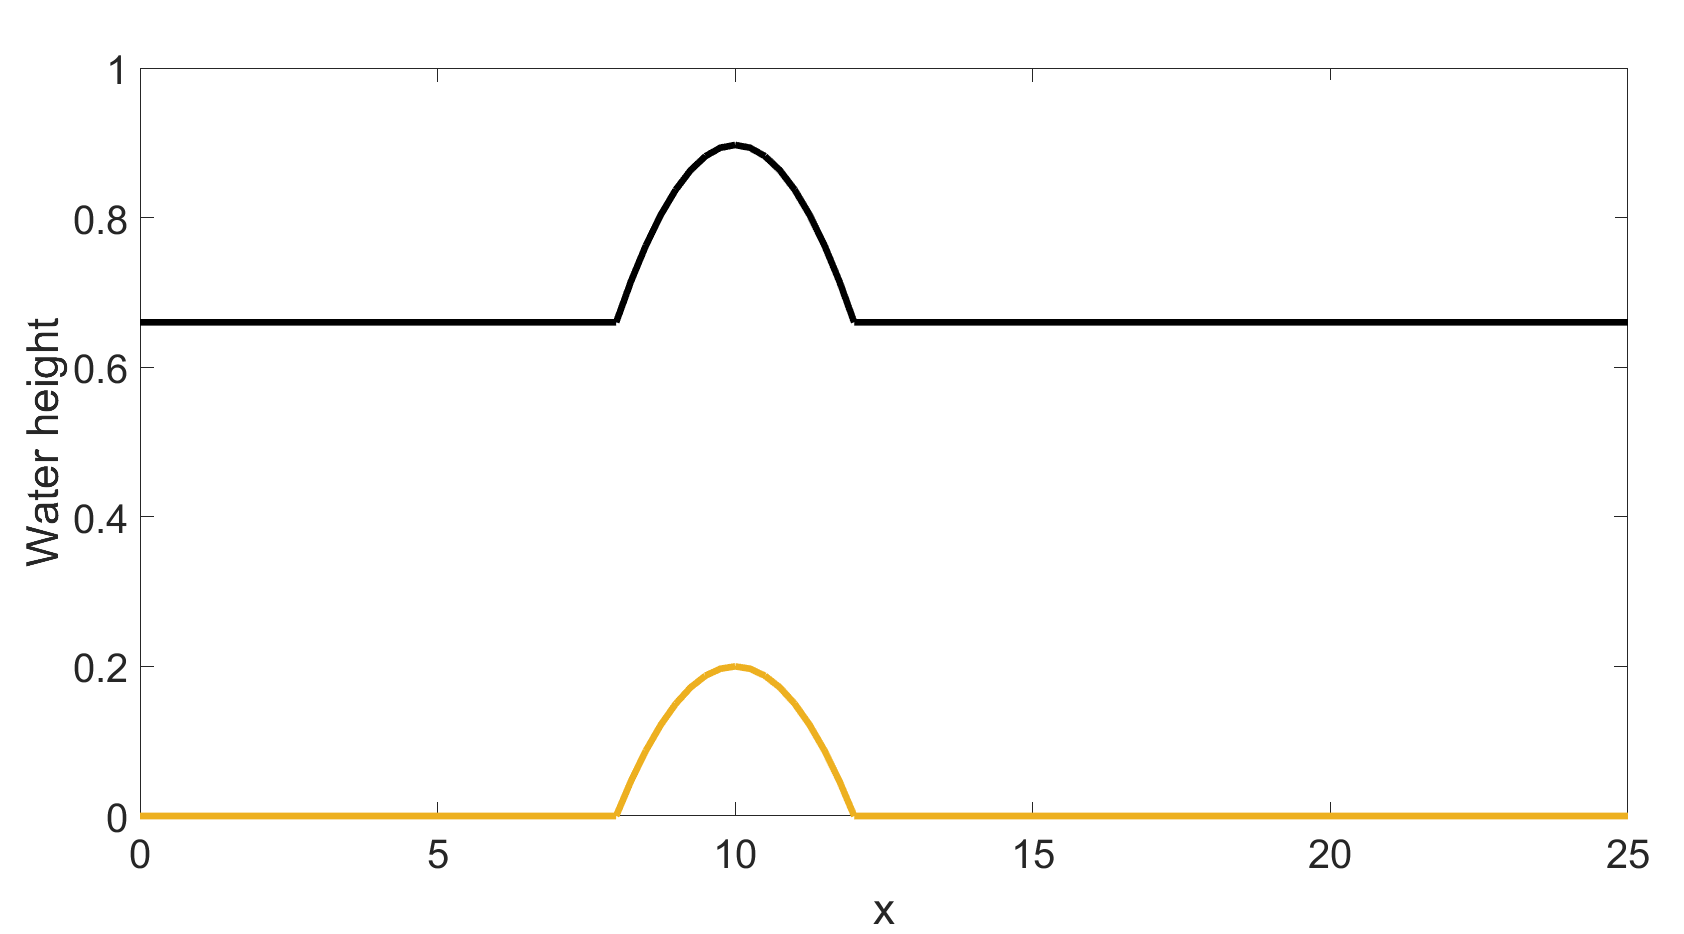
\includegraphics[width=3.5cm,height=1.25cm]{./height_supercrit}\\
%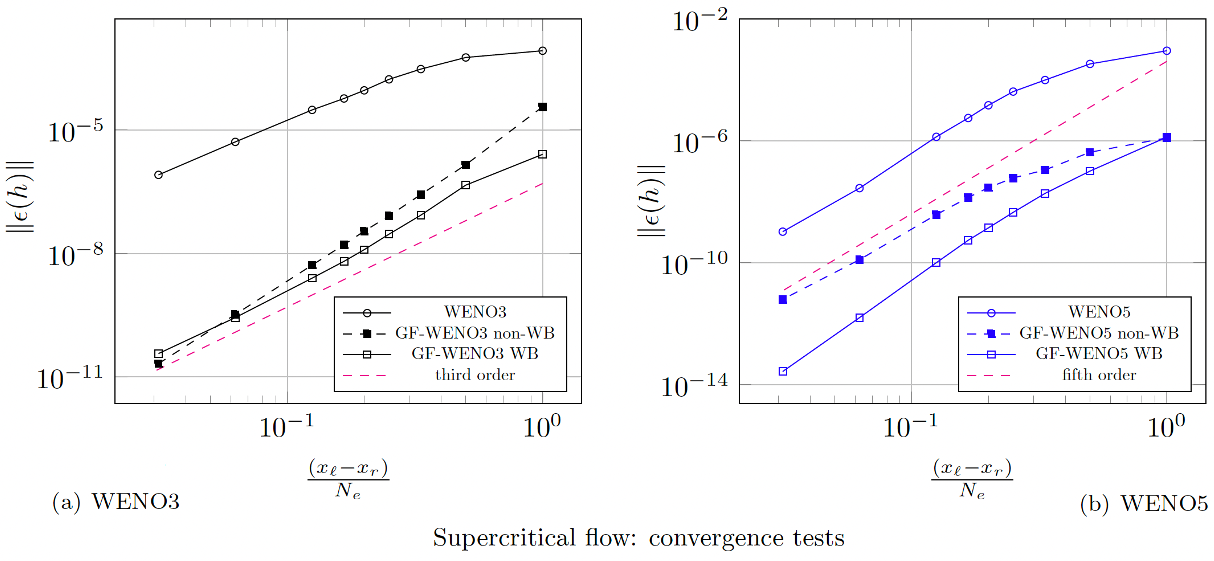
\includegraphics[width=0.6\textwidth]{./GF-FV-WENO-conv}
%\end{center}
Some options:
\begin{enumerate}
	\item The solution $U_i^*(x)$ of (1) if known or easy to find.
	\vspace{0.5cm}
	\item Solve (1) numerically w.r.t $U $ i.e $U_x = J(U)^{-1}S(U)H_x$
	\vspace{0.5cm}
	\item or.. 
\end{enumerate}
} 

%\only<4>{
%{\sf\small Small perturbation of steady state}\\
%\begin{center}
%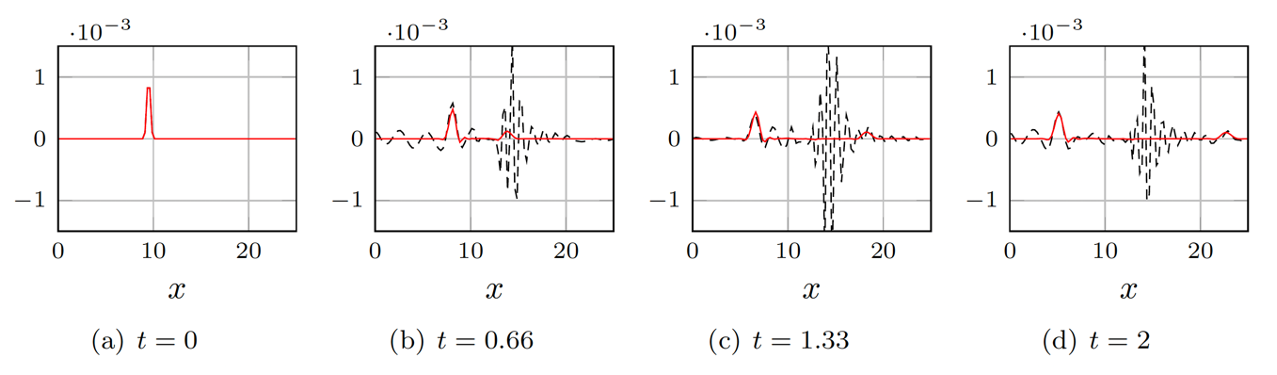
\includegraphics[width=0.9\textwidth]{./GF-WENO-FV-pert} 
%\end{center}
%} 
\end{frame}

%\begin{frame}{Global Flux Quadrature  with WENO approximation} 
	
%\only<4>{
%\begin{enumerate}
%\item[\textcolor{mblue1}{\Large\checkmark}] \textcolor{black}{No a-priori knowledge of equilibrium, all steady states!}  
%
%\vspace{0.2cm}
%
%\item[\textcolor{mblue1}{\Large\checkmark}] \textcolor{black}{No need of compute the solution of the Cauchy problem .. (maybe for initialization)}  
%
%\vspace{0.2cm}
%
%\item[\textcolor{mblue1}{\Large\checkmark}]  \textcolor{black}{Considerable accuracy enhancements at steady state (3 to 4 orders of magnitude)}
%
%\vspace{0.2cm}
%
%\item[\textcolor{red}{\Large$\times$}]  \textcolor{black}{No super convergence} 
%
%\vspace{0.2cm}
%
%\item[\textcolor{red}{\Large$\times$}]  \textcolor{black}{Very hard to charcterize the steady state and generate one }
%\end{enumerate}
%
%\begin{flushright}
%$ \overline{R}_i =R_{i-1/2}^+ - \sum_q \omega_q  \int_{x_{i-1/2}}^{x_q} S({\color{red}U_i(x)},\varphi(x)) dx$
%\end{flushright}
%}

%\end{frame}
 
 
\begin{frame}[t]{Global Flux Quadrature  with WENO approximation} 
\MyLogoa

 We seek solutions of the hyperbolic system of balance laws

\only<1-5>{\begin{equation}
	\partial_tU+\partial_x F(U)=  S(U)\partial_xH   \nonumber
	\vspace{0.25cm}
\end{equation}}

\only<6-17>{\begin{equation}
	\partial_tU+\partial_x \dfrac{U^2}{2}=  S(U) \partial_xH     \nonumber
	\vspace{0.25cm}
\end{equation}}
\only<18->{\begin{equation}
	\partial_t\bigg[\begin{array}{c} h\\hu\end{array}\bigg]+\partial_x\bigg[\begin{array}{c} hu\\hu^2 + gh^2/2\end{array}\bigg]=  - \bigg[\begin{array}{c} 0\\h\end{array}\bigg] b'(x)   \nonumber
%	\vspace{0.25cm}
\end{equation}}

%{\bf \textsf{New approach}} 


\only<1-2>{ \begin{equation*} 
 \dfrac{d U_i}{dt} + \dfrac{1}{\Delta x} \left( \widehat{G}_{i+1/2} - \widehat{G}_{i-1/2}   \right)   = 0  \nonumber
 \vspace{0.35cm}
\end{equation*}}
 
 \only<2>{
 
% \begin{enumerate}
% \item  \sout{Reconstruct  WENO polynomials  $U_i(x)$}
% 
% \vspace{0.15cm}
% 
% \item  Compute  nodal  source primitive $ R_i =R_{i-1} - \Delta x \sum_q \omega_q  S(U_{i-q},\varphi(x_{i-q}))$
% 
%  \vspace{0.15cm}
%  
%   \item  \sout{Compute  cell averaged fluxes  $ \overline{F}_i =  \sum_q \omega_q F({\color{red}U_i(x_q)},\varphi(x_q)) dx$}
%
%  \vspace{0.15cm}
%    
% \item  Reconstruct  WENO polynomials  $G_{i+1/2}^{\pm}(x)= (F+R)^{\pm}_{i+1/2}(x)$ 
% 
%  \vspace{0.15cm}
%  
% \item  Compute upwind fluxes $\widehat{G}_{i+1/2} = P^+_{i+1/2} G^-_{i+1/2}(x_{i+1/2}) + P^-_{i+1/2} G_{i+1/2}^+(x_{i+1/2})$
% \end{enumerate}

In this approach we seek to embed directly in the discrete equation a consistency condition with a discrete approximation of the flux form of the Cauchy problem. So we integrate directly the latter with some approach. 
}



\only<3>{
\begin{block}{Main result}
 {\bf Proposition} (Discrete steady state). {\it     The  WENO-FD scheme with  global flux quadrature 
 preserves exactly \underline{continuous} discrete  steady states $U^*_i =U(F_i)$ with $F$  obtained by integrating the ODE
 $$
 F' = S(U(F)) \partial_x H 
 $$ 
using the  multi-step ODE integrator with weights $\{\omega_q\}_{q\ge 0}$  %\footnote{See e.g.  Theorem 7.10 in Hairer, Wanner and Norset, Solving Ordinary Differential Equations I., Springer 1993}:   
on   spatial slabs of size $\hh$. \\[2.pt]

If $U(F)$ is a one to one mapping,    $U^*(x)$  
 verifies the  consistency estimates of the multi-step scheme.
 }  
 \end{block}
 
 \vspace{0.5cm}
 
 \begin{flushright}
{\rm Multi-step schemes so far: Adams methods AB$n$ and AM$n$}
\end{flushright}
} 

\only<4>{
	\begin{enumerate}
		\item Compute approximations $R_{j} = R_{j-1} +\mathcal{I}_{j-1/2}(U), $  $ \forall i$ where 
		\textcolor{blue}{$$ \mathcal{I}_{j-1/2} \approx \int_{x_{j-1}}^{x_j} S(U)H_x dx $$}
		\vspace{0.1cm}
		\item Define  \textcolor{red}{ $\mathcal{F}_j = F(U_j)-R_j$},  $j\in\{i-r-1,\cdots, i-s-1\}$
		\vspace{0.1cm}
		\item  Reconstruct  WENO polynomials  $G_{i+1/2}^{\pm}(x) $ using  $\mathcal{F}_j$ 
		\vspace{0.1cm}
		\item Compute upwind fluxes $\widehat{G}_{i+1/2} = P^+_{i+1/2} G^-_{i+1/2}(x_{i+1/2}) + P^-_{i+1/2} G_{i+1/2}^+(x_{i+1/2})$
	\end{enumerate}  
\vspace{0.1cm} 
\textcolor{red}{Difference with exactly well balanced:  The way in which the reference flux subtracted is obtained- Integration of the source}
}

\only<5>{
Here we compute 	$$ \mathcal{I}_{j-1/2} \approx \int_{x_{j-1}}^{x_j} S(U)H_x dx $$ using Adams ODE Integrators ie:
$$
\mathcal{I}_{j-1/2} = \sum_{k=-m1}^{m2}\beta_kS(U_{j+k})H_x(x_{j+k})
$$
Since we will work with schemes of formal accuracy $2k + 1 \ge 3$ we consider ODE solvers whose solutions have accuracy ar least $2k + 2 \ge 4$.
\vspace{0.1cm}	
\begin{itemize}
	\item Adams-Bashforth : $m_1=4,6,8$ and $m_2=-1$ 
	\vspace{0.1cm}
	\item Adams-Moulton:    $m_1=3,5,7$ and $m_2=0$ 
\end{itemize}
	}


\only<6>{
	\textbf{Moving solution} (safety check):   $S(U)=U-C$ and $H(x,t)=e^{-(x-x_0-Ct)^2}$, $U_{\text{ex}}=H(x,t)$  \\[5pt] %The wave is centered at $x_0=0.5$.   \\[5pt]
	
	\begin{minipage}{0.5\textwidth}
		\centering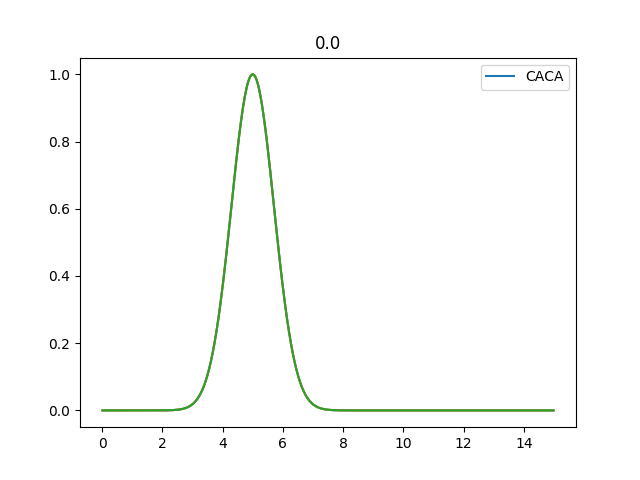
\includegraphics[width=0.8\textwidth]{figs/WENO-FD/figures/Burgers/MMS/initial} 
	\end{minipage}\hfill
	\begin{minipage}{0.5\textwidth}
%		 \begin{flushright}
		 For WENOn-ABm or  
		 WENOn-AMn \\[5pt] we expect  convergence rates $$\epsilon = \Delta x^{\min(m,n)}$$  
%		 \end{flushright}
	\end{minipage}
	}

\only<7>{
	\textbf{Moving solution} (safety check):   $S(U)=U-C$ and $H(x,t)=e^{-(x-x_0-Ct)^2}$, $U_{\text{ex}}=H(x,t)$  \\[5pt] %The wave is centered at $x_0=0.5$.   \\[5pt]
	
	
	\begin{minipage}{0.5\textwidth}
		\centering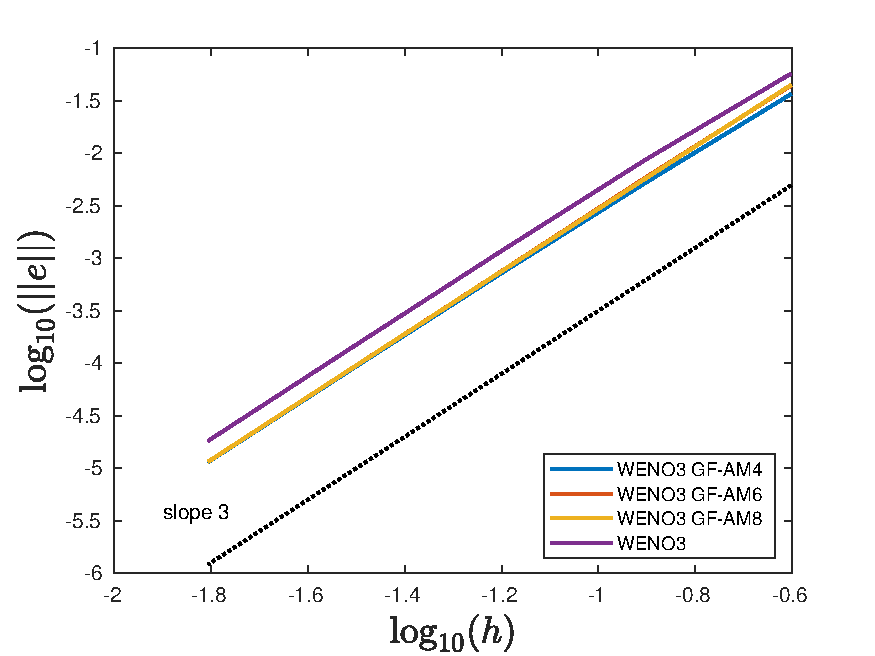
\includegraphics[width=0.85\textwidth]{figs/WENO-FD/figures/Burgers/MMS/weno3_AM_MMS_conv} 
	\end{minipage}\hfill
	\begin{minipage}{0.5\textwidth}
		\centering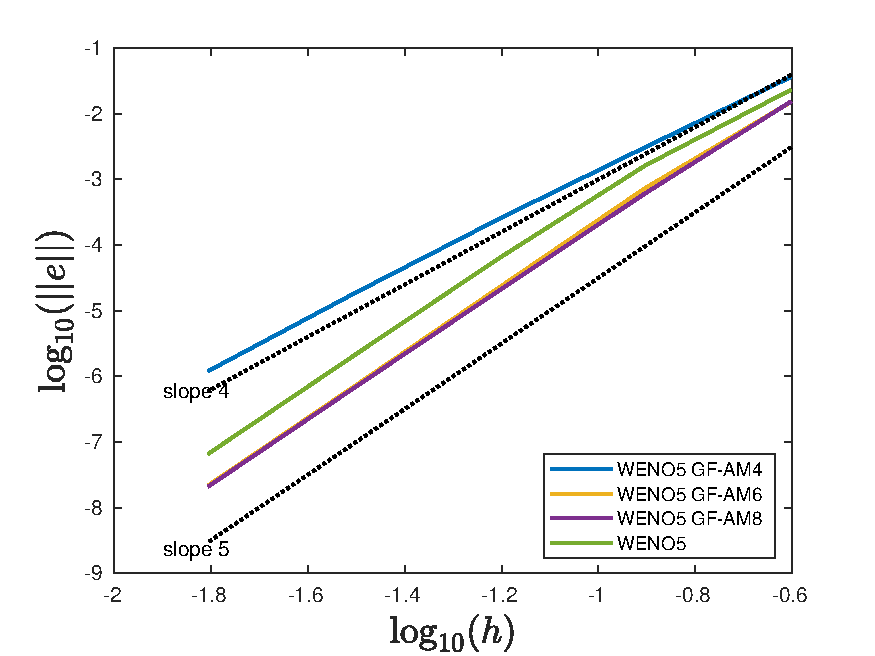
\includegraphics[width=0.85\textwidth]{figs/WENO-FD/figures/Burgers/MMS/weno5_AM_MMS_conv} 
	\end{minipage}
}


\only<8>{
	\textbf{Moving solution} (safety check):   $S(U)=U-C$ and $H(x,t)=e^{-(x-x_0-Ct)^2}$, $U_{\text{ex}}=H(x,t)$   \\[5pt] %The wave is centered at $x_0=0.5$.   \\[5pt]
	
	
	\begin{minipage}{0.5\textwidth}
		\centering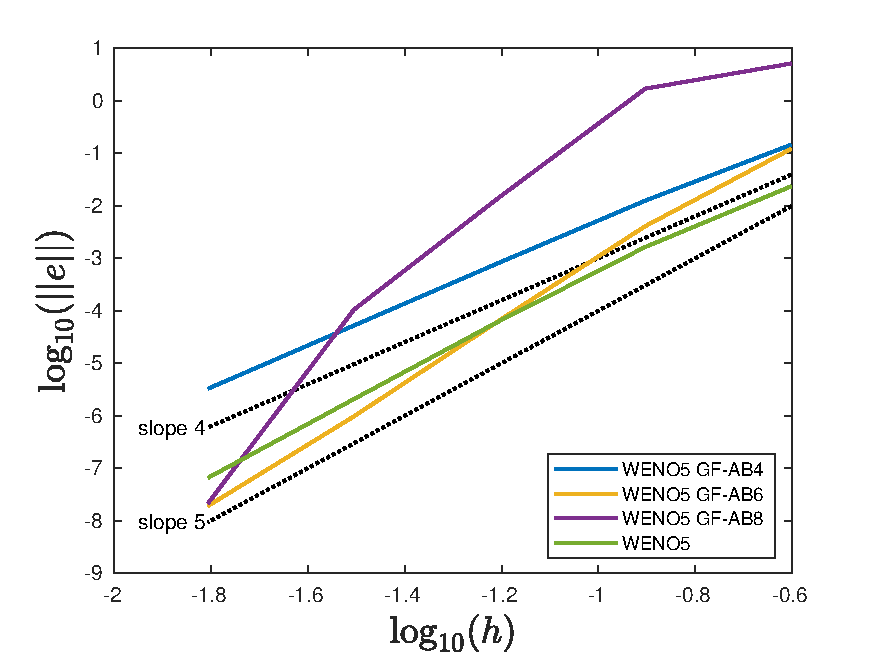
\includegraphics[width=0.8\textwidth]{figs/WENO-FD/figures/Burgers/MMS/weno5_AB_MMS_conv} 
	\end{minipage}\hfill
	\begin{minipage}{0.5\textwidth}
		\centering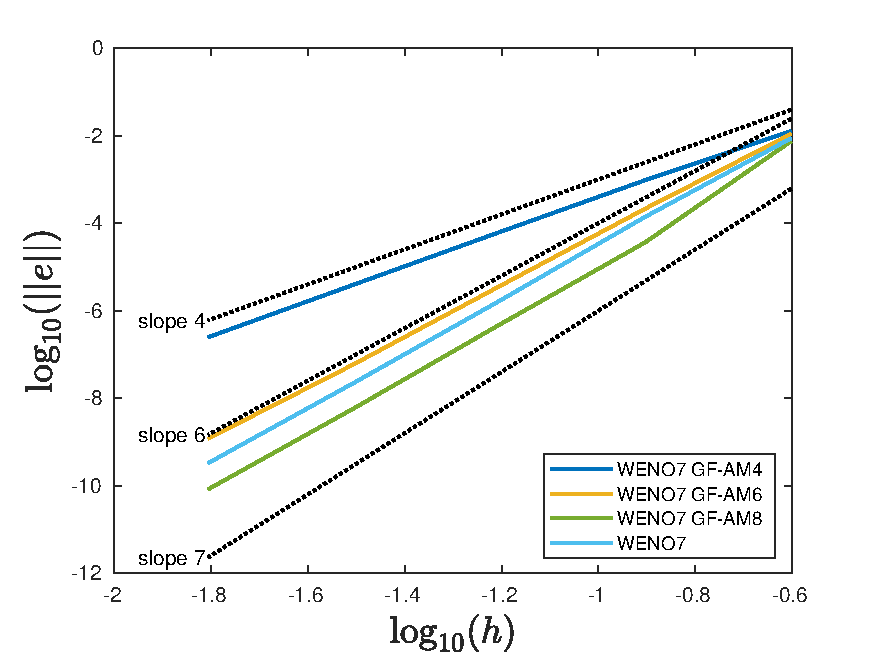
\includegraphics[width=0.85\textwidth]{figs/WENO-FD/figures/Burgers/MMS/weno7_AM_MMS_conv} 
	\end{minipage}
} 
 


 \only<9>{
\textbf{Steady state}: $S(U)=U^2$ and $H(x)=x$, exact solution  $U_{\text{ex}}(x)=e^x$ \\[10pt]


\begin{minipage}{0.5\textwidth}
\centering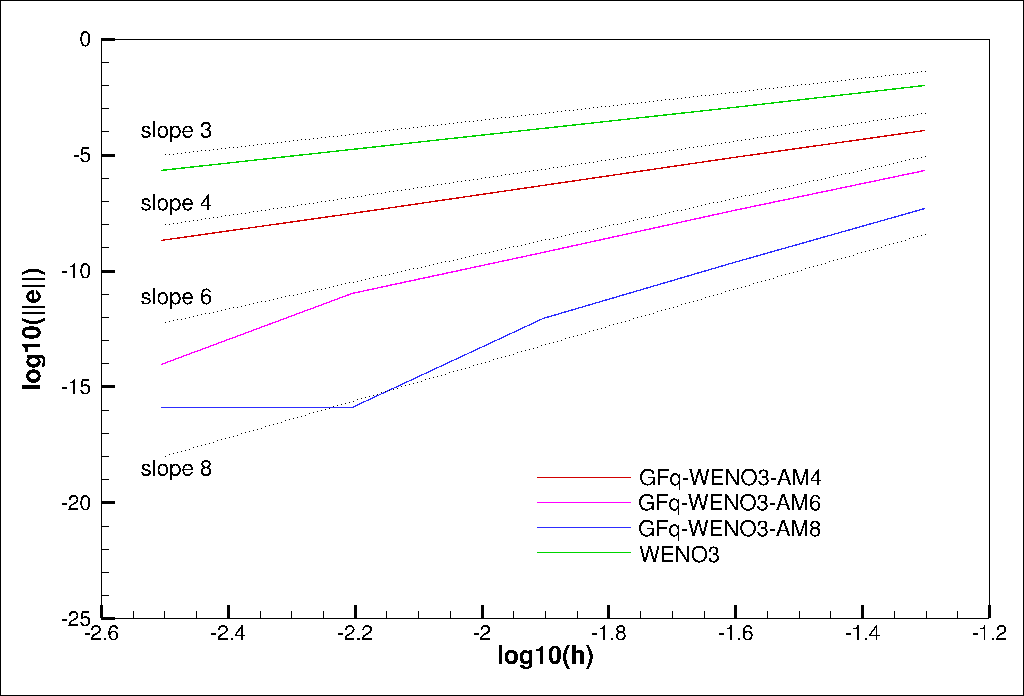
\includegraphics[width=0.8\textwidth]{figs/WENO-FD/figures/Burgers/convergence_steady/convburg-weno3} 
\end{minipage}\hfill
\begin{minipage}{0.5\textwidth}
\centering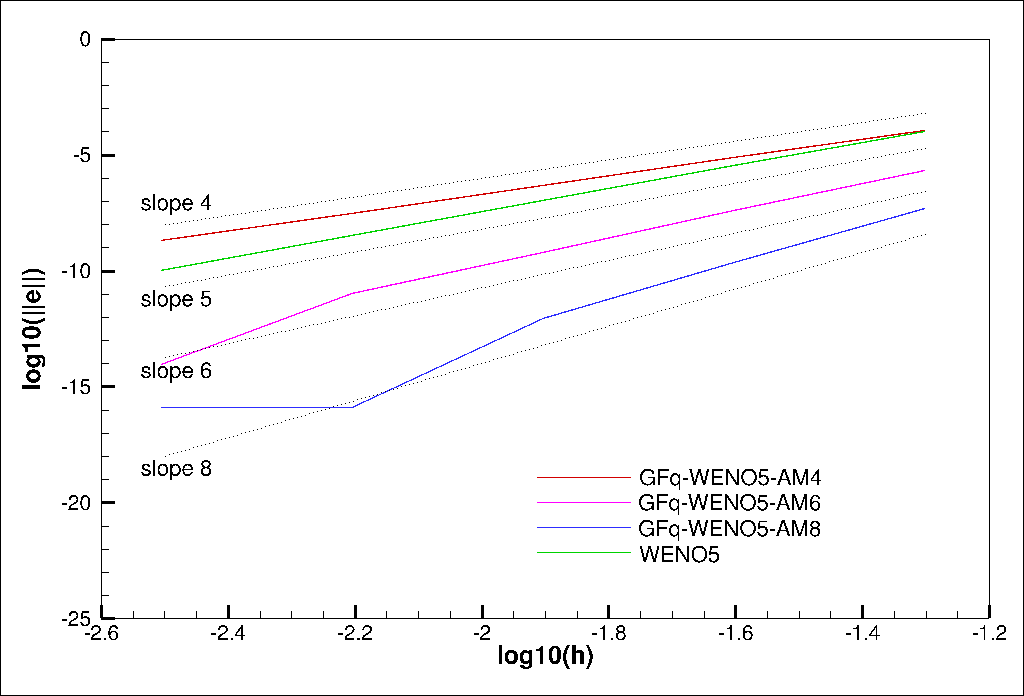
\includegraphics[width=0.8\textwidth]{figs/WENO-FD/figures/Burgers/convergence_steady/convburg-weno5}
\end{minipage}
} 

\only<10>{
Steady state: $S(U)=U^2$ and $\varphi=x+100\sin x$\\[5pt]


\begin{minipage}{0.5\textwidth}
\centering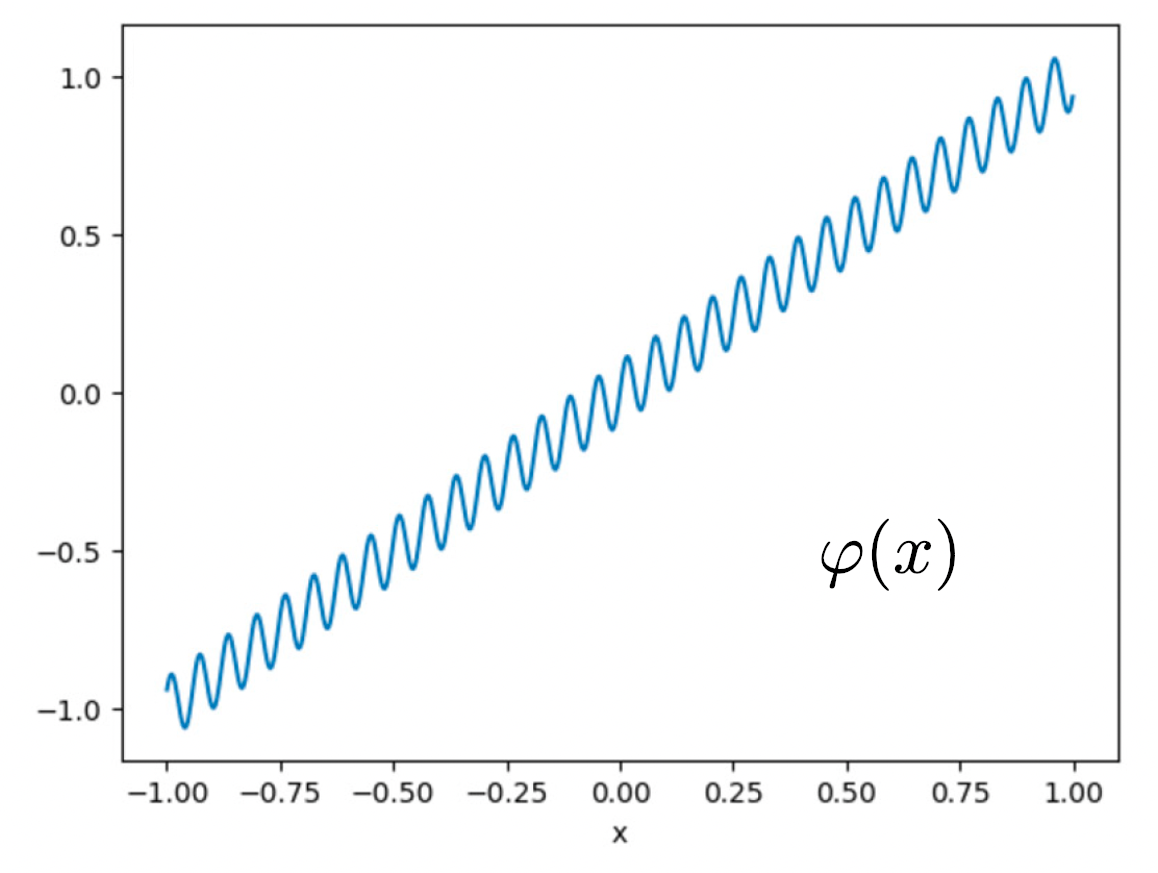
\includegraphics[width=0.8\textwidth]{figs/WENO-FD/figures/Burgers/perturbations/oscillation} 
\end{minipage}\hfill
\begin{minipage}{0.5\textwidth}
\centering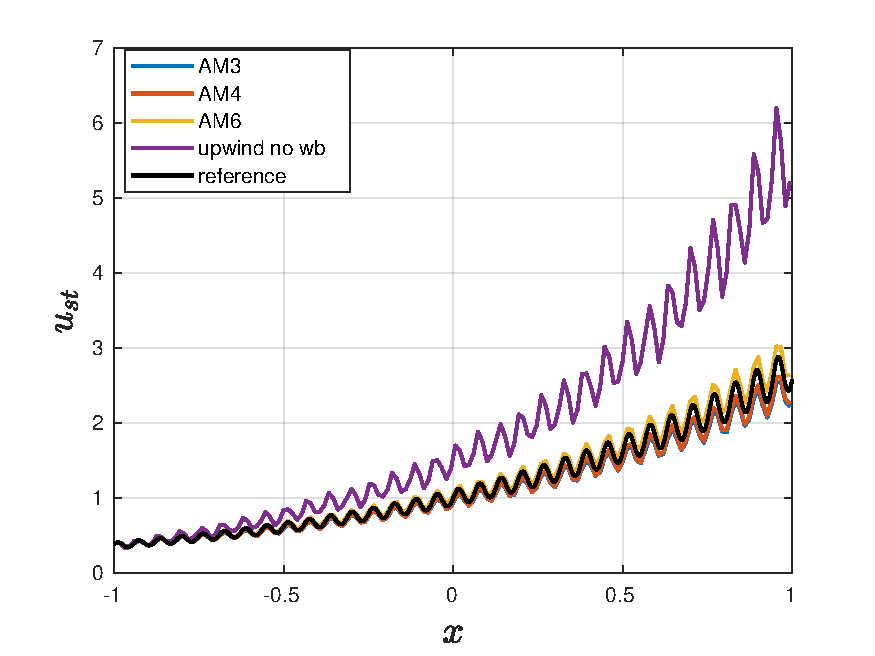
\includegraphics[width=0.85\textwidth]{figs/WENO-FD/figures/Burgers/perturbations/weno3_AM_stationary_n150} 
\end{minipage}
} 


\only<11>{
\textbf{Perturbed steady state}: $S(U)=U^2$ and $\varphi=x+100\sin x$ + top hat  $\delta u=0.2\chi_{[-0.7,-0.5]}$    \\[5pt]


\begin{minipage}{0.5\textwidth}
\centering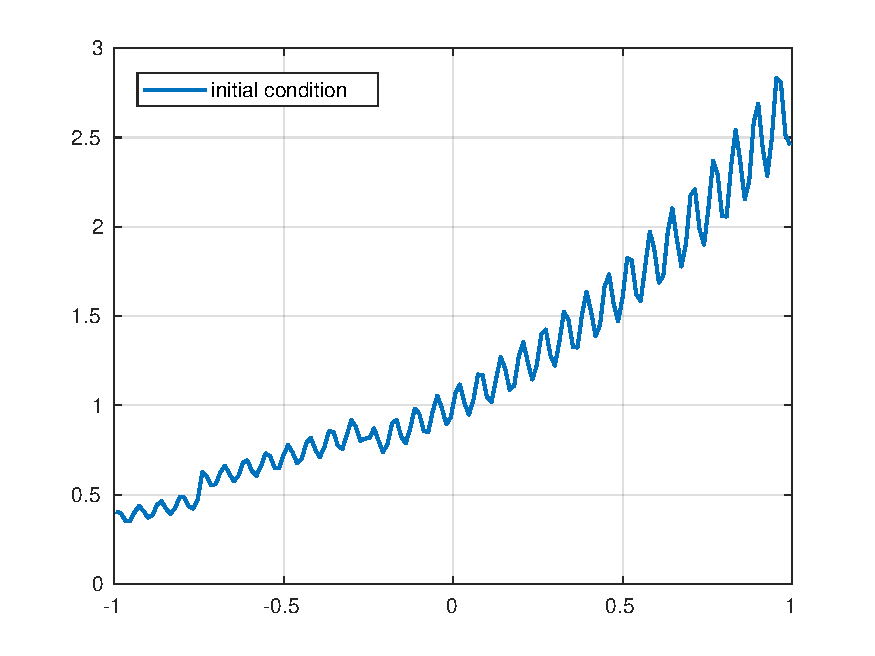
\includegraphics[width=0.8\textwidth]{figs/WENO-FD/figures/Burgers/perturbations/initial_cond_DISC_n150} 
\end{minipage}\hfill
\begin{minipage}{0.5\textwidth}
\centering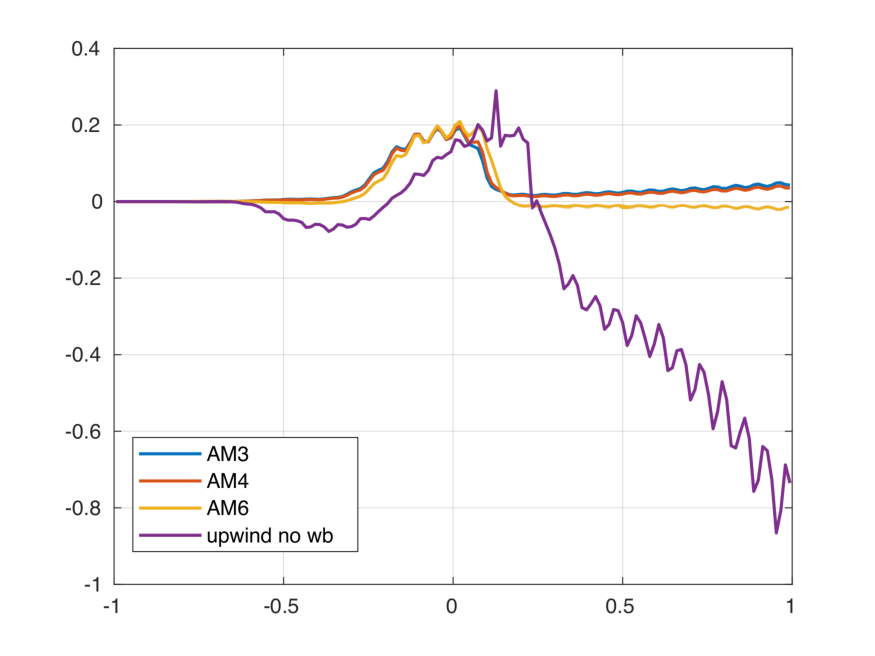
\includegraphics[width=0.85\textwidth]{figs/WENO-FD/figures/Burgers/perturbations/weno3_AM_DISC_n150} 
\end{minipage}
}

\only<12>{
	\textbf{Perturbed steady state}: $S(U)=U^2$ and $\varphi=x+100\sin x$ + top hat  $\delta u=0.2\chi_{[-0.7,-0.5]}$    \\[5pt]
	
	
	\begin{minipage}{0.5\textwidth}
		\centering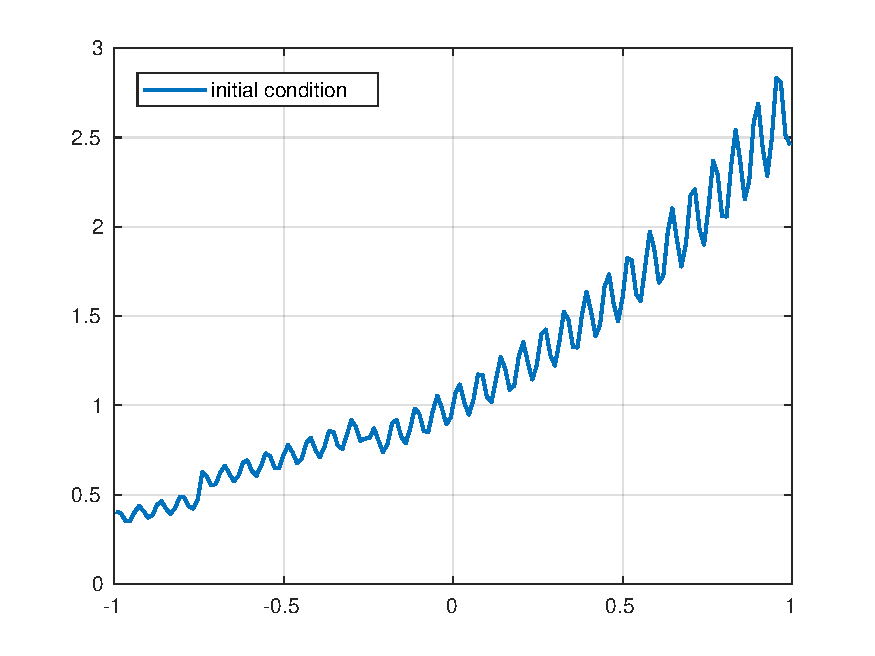
\includegraphics[width=0.8\textwidth]{figs/WENO-FD/figures/Burgers/perturbations/initial_cond_DISC_n150} 
	\end{minipage}\hfill
	\begin{minipage}{0.5\textwidth}
		\centering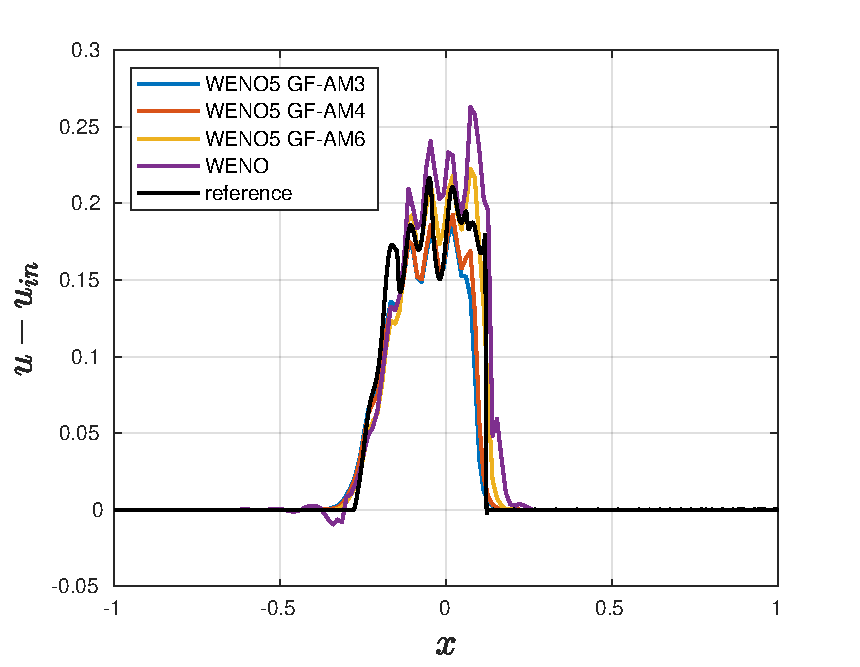
\includegraphics[width=0.85\textwidth]{figs/WENO-FD/figures/Burgers/perturbations/weno5_AM_DISC_n150} 
	\end{minipage}
}

\only<13>{
\textbf{Perturbed steady state}: $S(U)=U^2$ and $\varphi=x+100\sin x$ +   Gaussian with amplitude $\alpha=0.005$    \\[5pt]
	
	
	\begin{minipage}{0.5\textwidth}
		\centering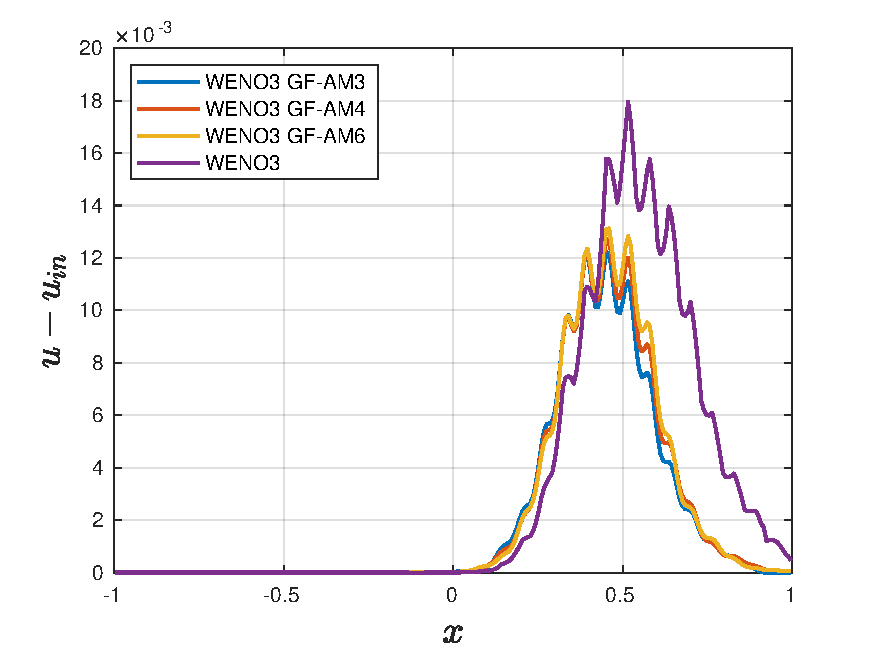
\includegraphics[width=0.85\textwidth]{figs/WENO-FD/figures/Burgers/perturbations/weno3_AM_error_pert0p005} 
	\end{minipage}\hfill
	\begin{minipage}{0.5\textwidth}
		\centering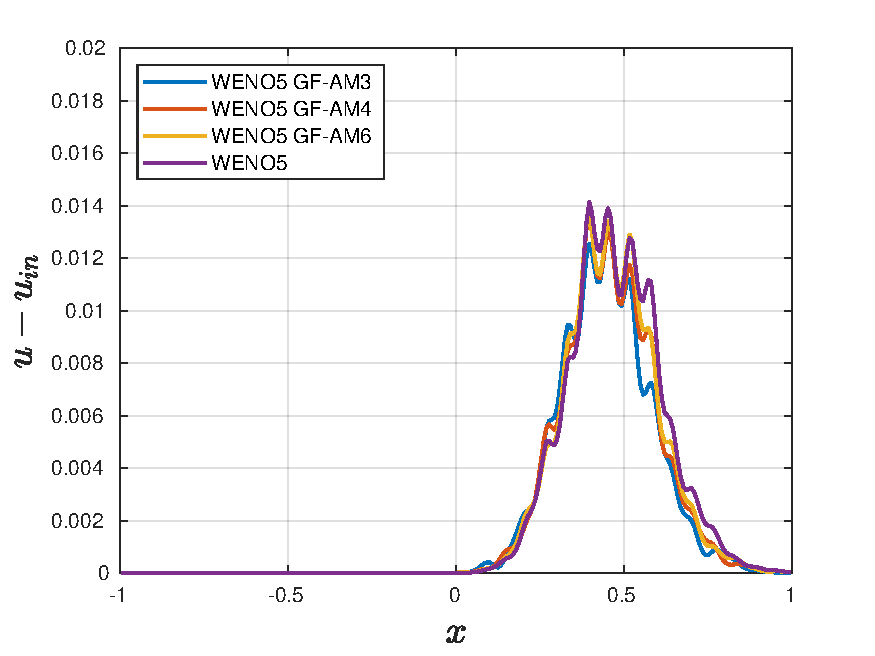
\includegraphics[width=0.85\textwidth]{figs/WENO-FD/figures/Burgers/perturbations/weno5_AM_error_pert0p005} 
	\end{minipage}
}


\only<14>{
	\textbf{Discontinuous H}:
	 $S(U)=U^2,$ $H(x)=0.1x|_{(x \le 0)}, 0.9+x|_{(x > 0.5)}, (0.5+x)|_{(0< x \le 0.5)},$ $U_{\text{ex}}(x)=e^H$  \\[5pt]
	
		\begin{minipage}{0.5\textwidth}
			\centering\includegraphics[width=0.85\textwidth]{figs/WENO-FD/figures/Burgers/Hdisc/nocorrection/weno3_am4_noH} 
		\end{minipage}\hfill
		\begin{minipage}{0.5\textwidth}
			\centering\includegraphics[width=0.85\textwidth]{figs/WENO-FD/figures/Burgers/Hdisc/nocorrection/weno5_am8_noH} 
		\end{minipage}
}


\only<15>{
	\textbf{Discontinuous H}: $S(U)=U^2,$ $H(x)=0.1x|_{(x \le 0)}, 0.9+x|_{(x > 0.5)},$ $U_{\text{ex}}(x)=e^H$  \\[5pt]  
	Lets assume that the discontinuity is at the middle of the cell $[x_{i-1},\; x_{i}]$  
	\begin{itemize}
		\item  Far from the discontinuity we use our standard $n$-step selected method. \\[8pt]
		\item In the cell  $[x_{i-1},\; x_{i}]$ we set $I_{i-1/2} = \tilde{S}_{i-1/2}[[H]]_{i-1/2}$ where $\tilde{S}_{i-1/2}$ linearization, such  as $[[F]]_{i-1/2} = \tilde{S}_{i-1/2}[[H]]_{i-1/2}$. \\[8pt]
		\item For $n$ cells after the discontinuity we use AM2.
	\end{itemize}
	
%	\begin{minipage}{0.5\textwidth}
%		\centering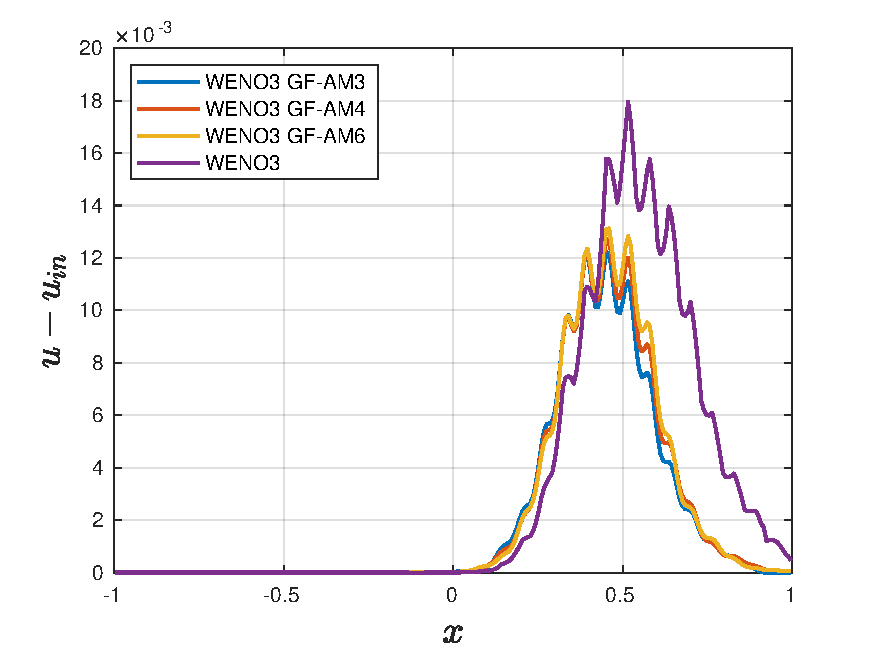
\includegraphics[width=0.85\textwidth]{figs/WENO-FD/figures/Burgers/perturbations/weno3_AM_error_pert0p005} 
%	\end{minipage}\hfill
%	\begin{minipage}{0.5\textwidth}
%		\centering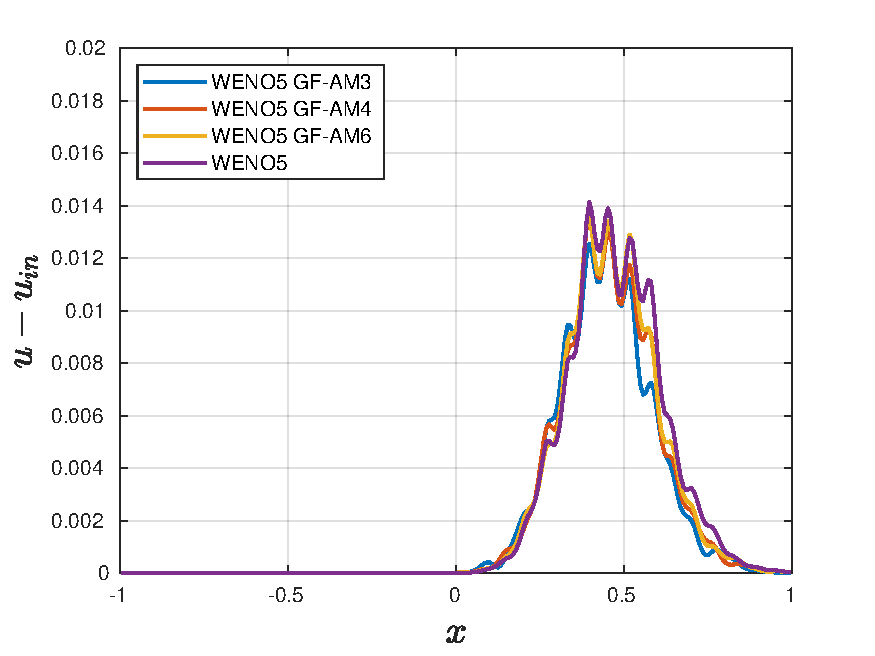
\includegraphics[width=0.85\textwidth]{figs/WENO-FD/figures/Burgers/perturbations/weno5_AM_error_pert0p005} 
%	\end{minipage}
}

\only<16>{
	\textbf{Discontinuous H}: $S(U)=U^2,$ $H(x)=0.1x|_{(x \le 0)}, 0.9+x|_{(x > 0.5)},$ $U_{\text{ex}}(x)=e^H$  \\[5pt]

	\begin{minipage}{0.5\textwidth}
		\centering\includegraphics[width=0.85\textwidth]{figs/WENO-FD/figures/Burgers/Hdisc/N100_t0p3} 
	\end{minipage}\hfill
	\begin{minipage}{0.5\textwidth}
		\centering\includegraphics[width=0.85\textwidth]{figs/WENO-FD/figures/Burgers/Hdisc/N100_t0p5} 
	\end{minipage}
}


\only<17>{
	\textbf{Discontinuous H}: $S(U)=U^2,$ $H(x)=0.1x|_{(x \le 0)}, 0.9+x|_{(x > 0.5)},$ $U_{\text{ex}}(x)=e^H$  \\[5pt] 
	
	\begin{minipage}{0.5\textwidth}
		\centering\includegraphics[width=0.85\textwidth]{figs/WENO-FD/figures/Burgers/Hdisc/N300_t0p3} 
	\end{minipage}\hfill
	\begin{minipage}{0.5\textwidth}
		\centering\includegraphics[width=0.85\textwidth]{figs/WENO-FD/figures/Burgers/Hdisc/N300_t0p5} 
	\end{minipage}
}



\only<18>{
\textbf{Lake at rest on a parabolic hump}. \\[5pt]
\begin{minipage}{0.5\textwidth}
\centering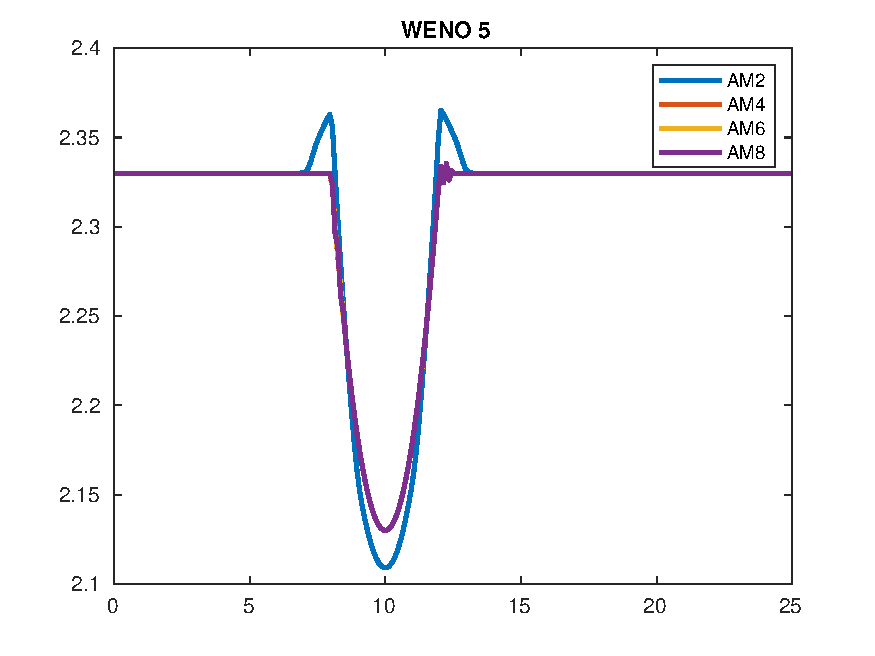
\includegraphics[width=0.8\textwidth]{figs/WENO-FD/figures/SW/lake_at_rest/weno5_N250_eta} 
\end{minipage}\hfill
\begin{minipage}{0.5\textwidth}
\centering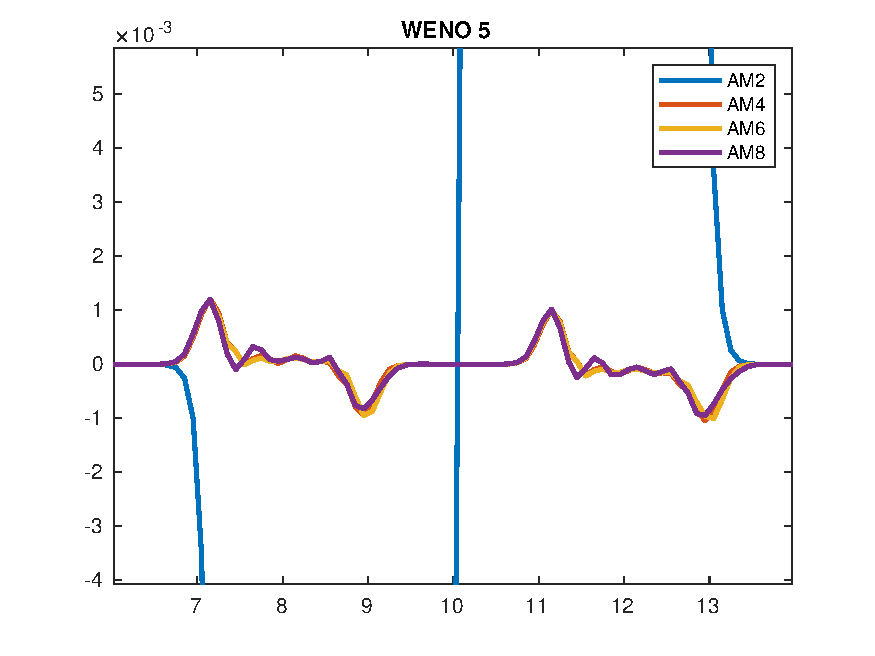
\includegraphics[width=0.8\textwidth]{figs/WENO-FD/figures/SW/lake_at_rest/weno5_N250_q} 
\end{minipage}
}


\only<19>{
Method modification (with both AB and AM):
$$
\hat b(x) = \sum_{m}L_{m}(x) b(x_m)
$$
with  $\{x_m\}$ the points generating the AMm method. We  proceed as  follows  

$$
\int_{x_i}^{x_{i+1}}gh b'(x) dx \approx  
\int_{x_i}^{x_{i+1}}g\eta \hat b'(x) dx  - \int_{x_i}^{x_{i+1}} g \bigg( \dfrac{\hat b^2}{2}\bigg)'dx = g \sum_m \omega_m \eta_m \hat b'(x_m) - g\bigg( \dfrac{ b^2_{i+1}}{2}-\dfrac{ b^2_{i}}{2} \bigg)
$$

}


\only<20>{
For lake at rest: \\
\vspace{0.5cm}
Then it easy to show that 
$$
\begin{aligned}
	F_{i+1} - F_i +   g \sum_m \omega_m \eta_m \hat b'(x_m) - g\bigg( \dfrac{ b^2_{i+1}}{2}-\dfrac{ b^2_{i}}{2} \bigg) =0 
\end{aligned}
$$
%$$
%\begin{aligned}
%F_{i+1} - F_i +   g \sum_m \omega_m \eta_m \hat b'(x_m) - g\bigg( \dfrac{ b^2_{i+1}}{2}-\dfrac{ b^2_{i}}{2} \bigg) &=\\ 
%g\bigg( \dfrac{ h^2_{i+1}}{2}-\dfrac{ h^2_{i}}{2} \bigg)  
%+g \eta_0 \sum_m \omega_m \hat b'(x_m)- g\bigg( \dfrac{ b^2_{i+1}}{2}-\dfrac{ b^2_{i}}{2} \bigg) &=\\
% g\bigg( \dfrac{ (\eta_0-b_{i+1})^2}{2}-\dfrac{ (\eta_0-b_i)^2}{2} \bigg)  +g \eta_0 \int_{x_i}^{x_{i+1}} \hat b'(x)dx - g\bigg( \dfrac{ b^2_{i+1}}{2}-\dfrac{ b^2_{i}}{2} \bigg) &=\\
% -g\eta_0(b_{i+1}-b_i)+   g\bigg( \dfrac{ b^2_{i+1}}{2}-\dfrac{ b^2_{i}}{2} \bigg)+   g\eta_0(b_{i+1}-b_i) - g\bigg( \dfrac{ b^2_{i+1}}{2}-\dfrac{ b^2_{i}}{2} \bigg) &= 0
%\end{aligned}
%$$


}



\only<21>{
	\textbf{Lake at rest}\\
	\begin{minipage}{0.4\textwidth}
		\centering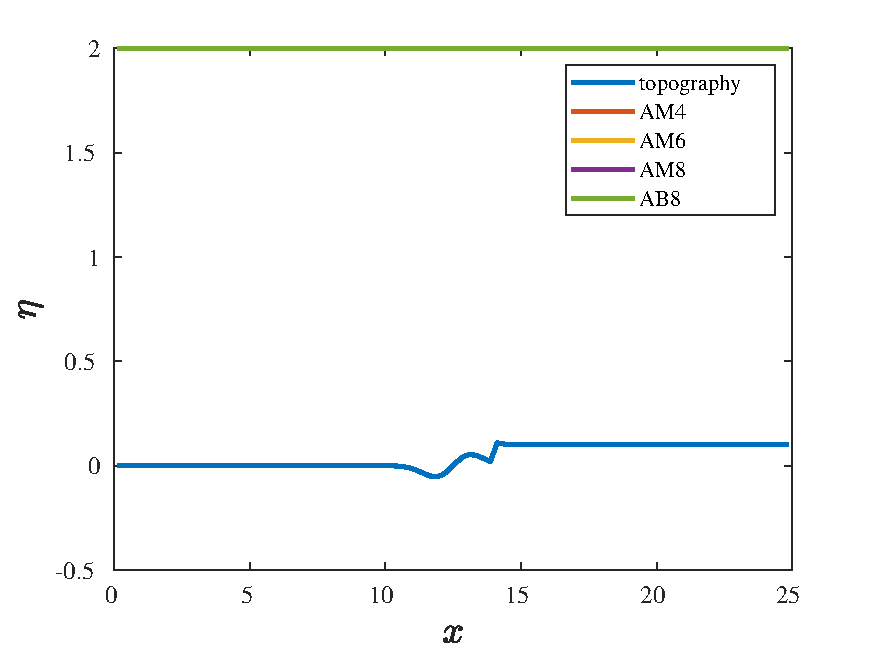
\includegraphics[width=\textwidth]{figs/WENO-FD/figures/SW/lake_at_rest/eta_lake_at_rest_b_reco} 
	\end{minipage}\hfill
	\begin{minipage}{0.5\textwidth}
		\centering\includegraphics[width=0.8\textwidth]{figs/WENO-FD/figures/SW/lake_at_rest/q_lake_at_rest_b_reco} 
	\end{minipage}
}



\only<22>{
\textbf{Lake at rest with perturbation}\\
\begin{minipage}{0.4\textwidth}
\centering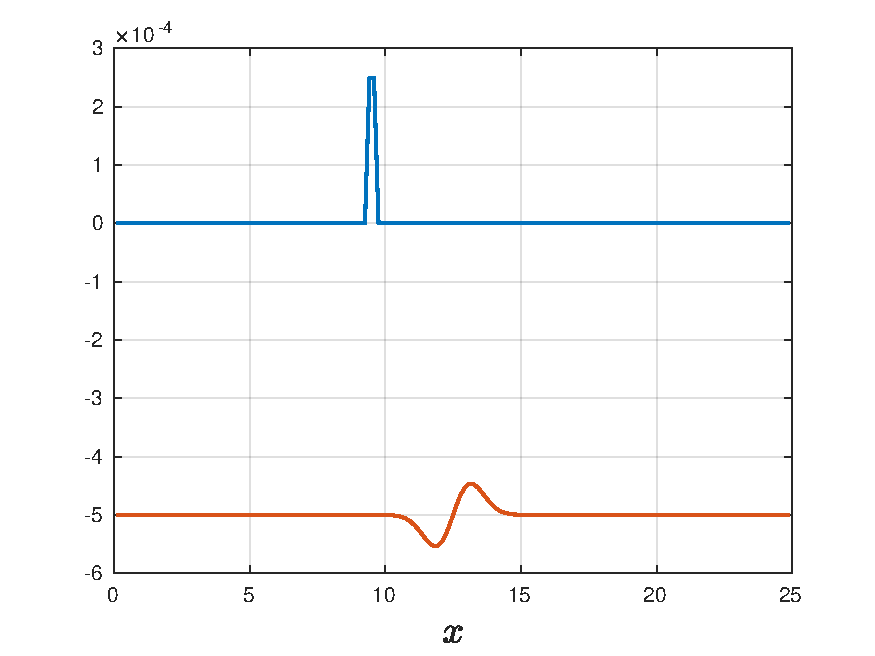
\includegraphics[width=\textwidth]{figs/WENO-FD/figures/SW/perturbations/weno3_lake_initial} 
\end{minipage}\hfill
\begin{minipage}{0.6\textwidth}
\centering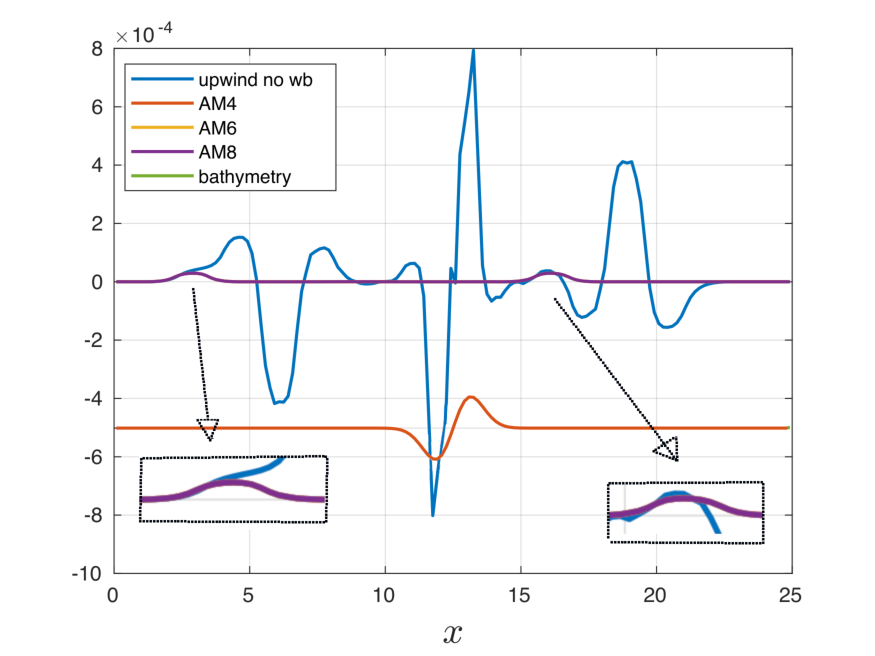
\includegraphics[width=0.8\textwidth]{figs/WENO-FD/figures/SW/perturbations/weno3_lake_t1p5-1} 
\end{minipage}
}


\only<23>{
\textbf{Supercritical flow on a smooth hump}\\
\begin{minipage}{0.4\textwidth}
\centering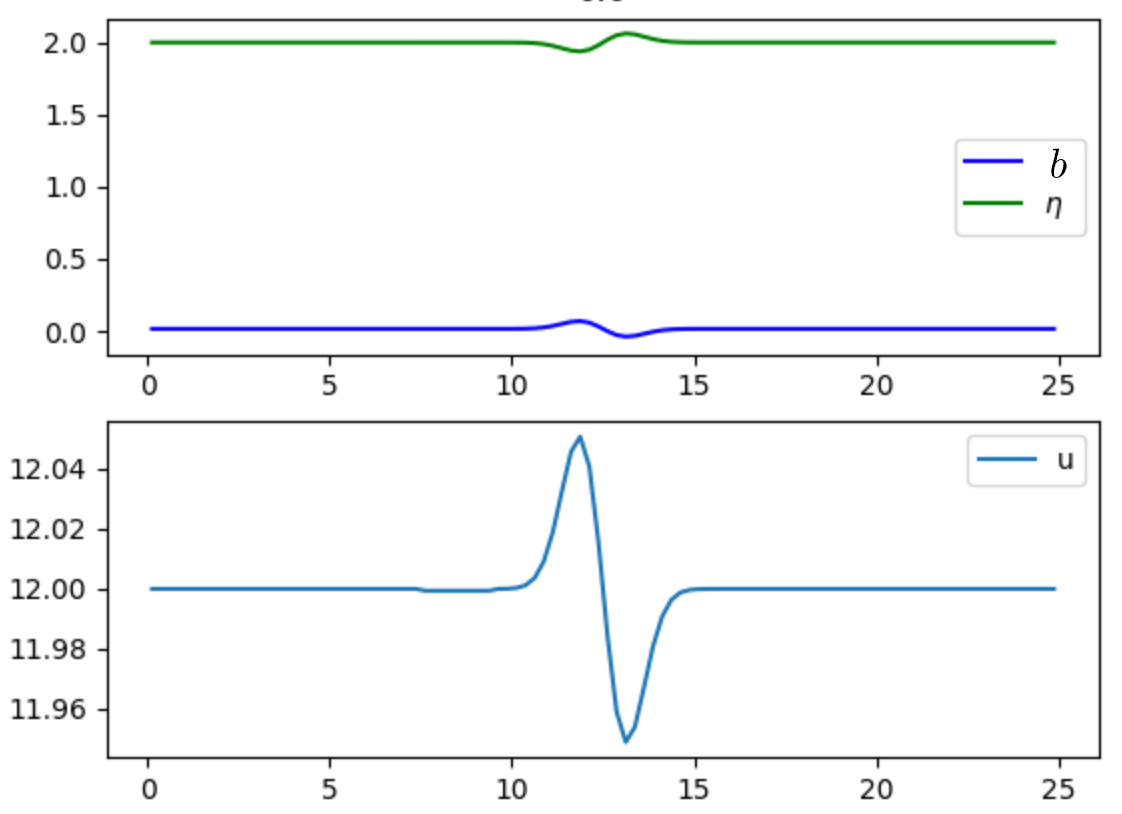
\includegraphics[width=\textwidth]{figs/WENO-FD/figures/SW/Supercritical/super-ini} 
\end{minipage}\hfill
\begin{minipage}{0.6\textwidth}
\centering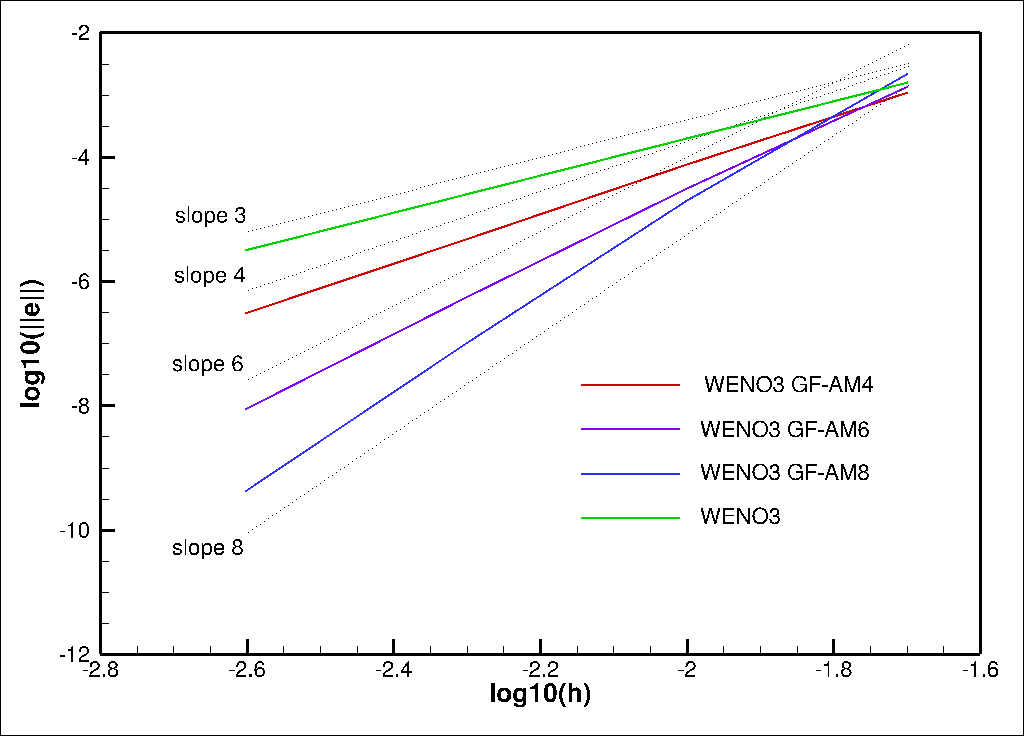
\includegraphics[width=0.8\textwidth]{figs/WENO-FD/figures/SW/Supercritical/conv} 
\end{minipage}
}

\only<24>{
\textbf{Supercritical flow with perturbation}\\
\begin{minipage}{0.5\textwidth}
\centering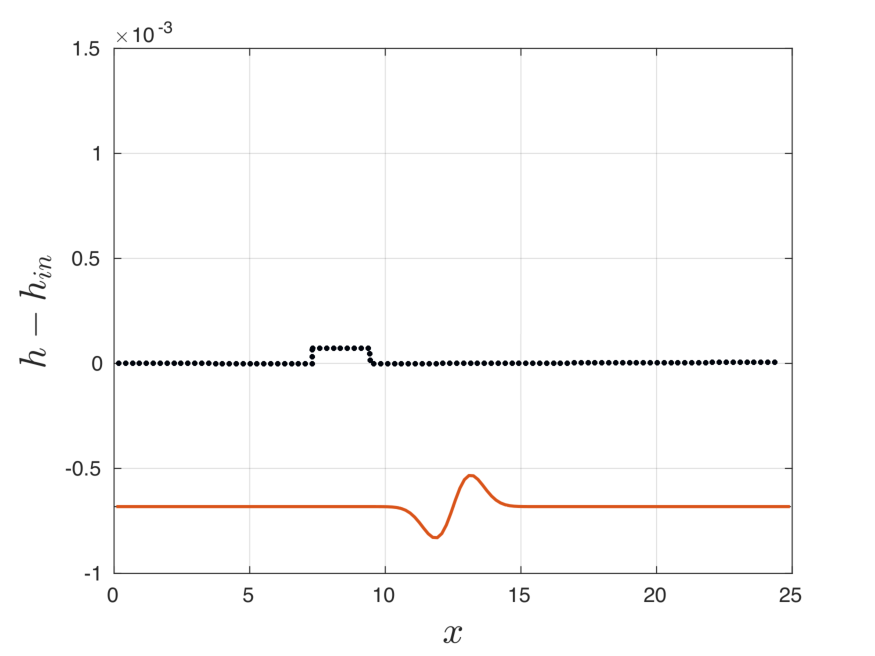
\includegraphics[width=0.9\textwidth]{figs/WENO-FD/figures/SW/perturbations/weno3_sup_DISCsmall_n100_error_ini}
\end{minipage}\hfill
\begin{minipage}{0.5\textwidth}
\centering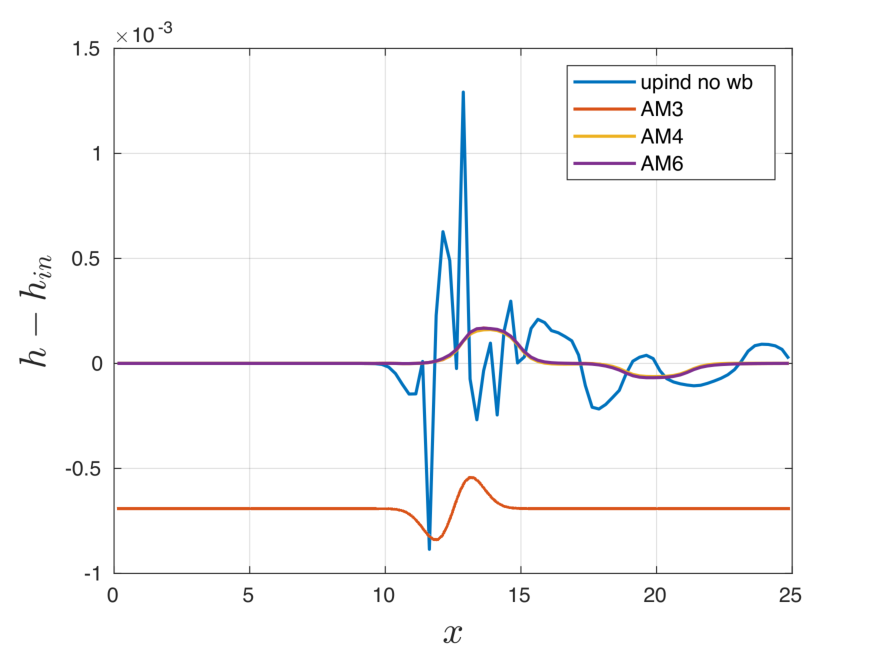
\includegraphics[width=0.9\textwidth]{figs/WENO-FD/figures/SW/perturbations/weno3_sup_DISCsmall_n100_error_h} 
\end{minipage}
}


\only<25>{
\textbf{Supercritical flow with perturbation}\\
\begin{minipage}{0.5\textwidth}
\centering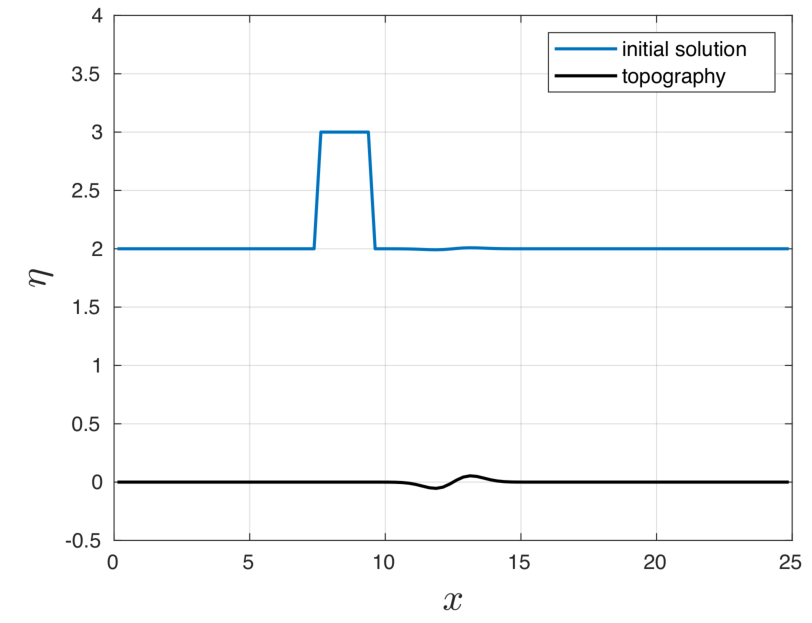
\includegraphics[width=0.9\textwidth]{figs/WENO-FD/figures/SW/perturbations/initial_discbig}
\end{minipage}\hfill
\begin{minipage}{0.5\textwidth}
\centering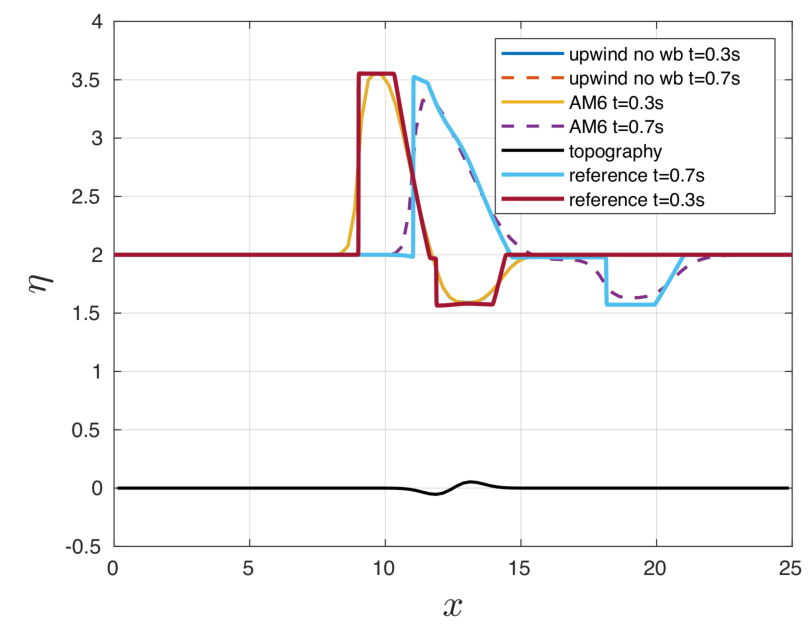
\includegraphics[width=0.9\textwidth]{figs/WENO-FD/figures/SW/perturbations/weno3_evolution_upAM61} 
\end{minipage}
}


\only<26>{
	\textbf{Subcritical flow on a smooth hump}\\
	\begin{minipage}{0.4\textwidth}
		\centering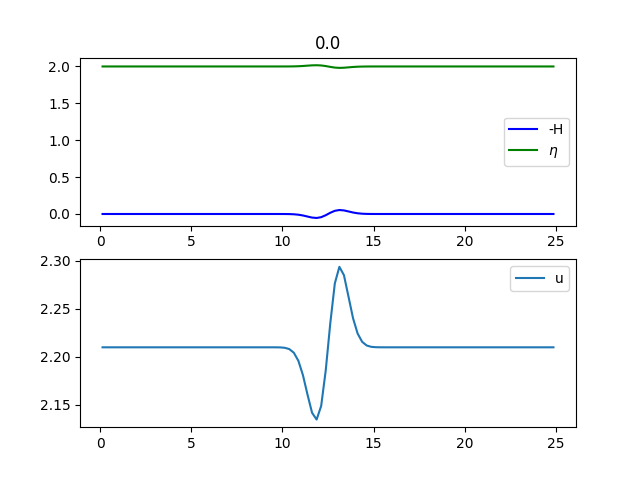
\includegraphics[width=\textwidth]{figs/WENO-FD/figures/SW/Subcritical/initial_con} 
	\end{minipage}\hfill
	\begin{minipage}{0.6\textwidth}
		\centering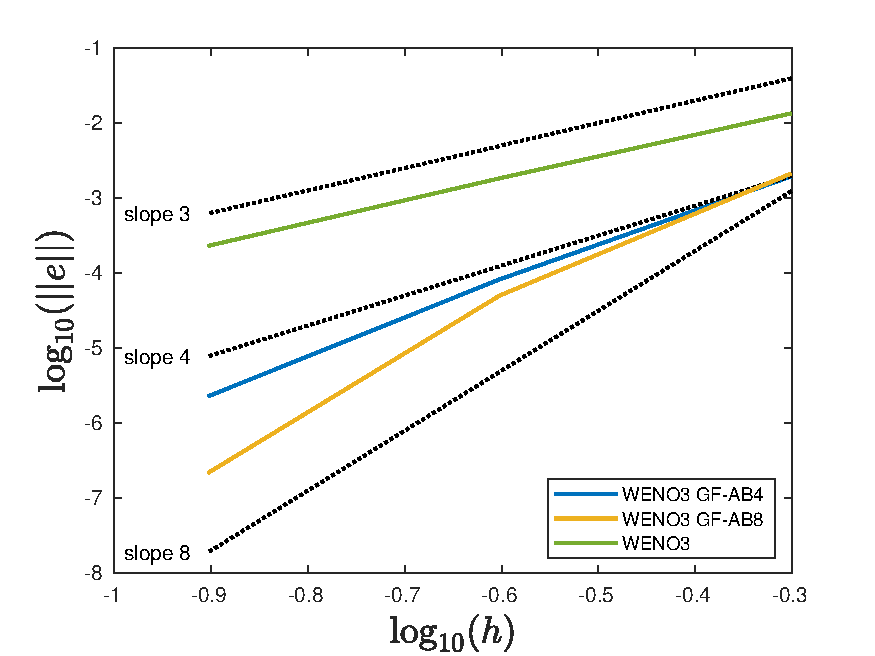
\includegraphics[width=0.8\textwidth]{figs/WENO-FD/figures/SW/Subcritical/weno3_AM_sub_conv} 
	\end{minipage}
}

\only<27>{
	\textbf{Subcritical flow with perturbation}\\
	\begin{minipage}{0.5\textwidth}
		\centering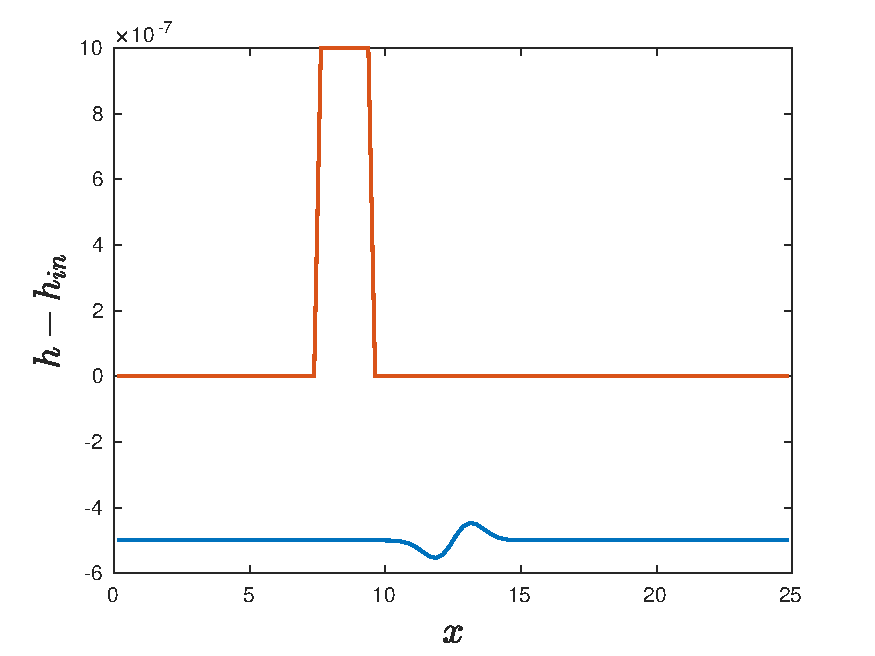
\includegraphics[width=0.9\textwidth]{figs/WENO-FD/figures/SW/perturbations/initial_sub_disc_small}
	\end{minipage}\hfill
	\begin{minipage}{0.5\textwidth}
		\centering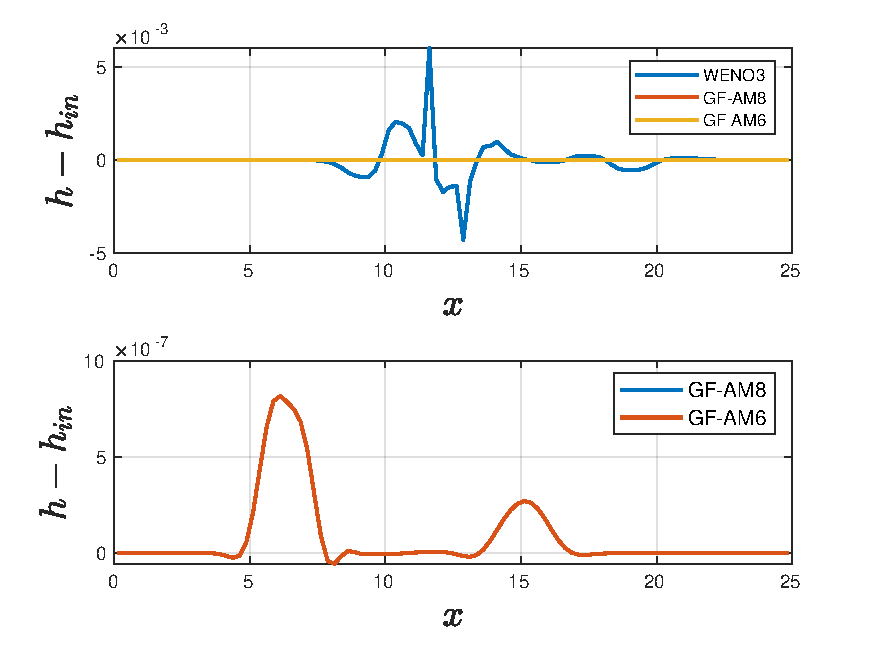
\includegraphics[width=0.9\textwidth]{figs/WENO-FD/figures/SW/perturbations/weno3_sub_DISCsmall_eta} 
	\end{minipage}
}

\only<28>{
	\textbf{Subcritical flow with perturbation}\\
	\begin{minipage}{0.5\textwidth}
		\centering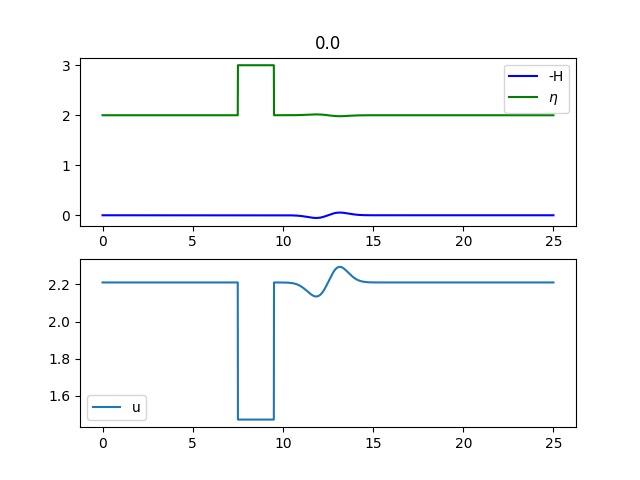
\includegraphics[width=0.9\textwidth]{figs/WENO-FD/figures/SW/perturbations/initial_big_sub}
	\end{minipage}\hfill
	\begin{minipage}{0.5\textwidth}
		\centering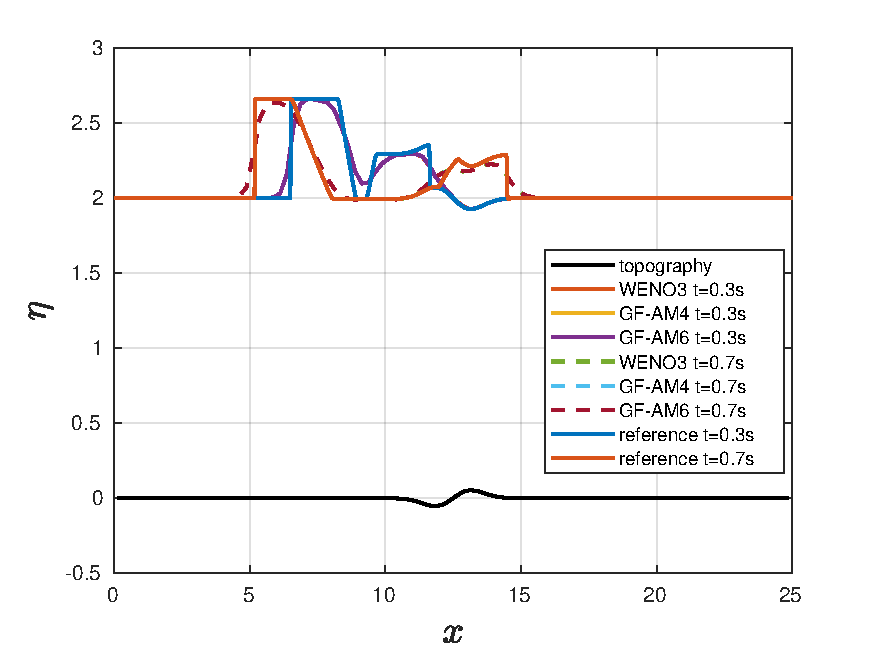
\includegraphics[width=0.9\textwidth]{figs/WENO-FD/figures/SW/perturbations/weno3_sub_DISCbig_eta} 
	\end{minipage}
}

\only<29>{
	\textbf{Subcritical flow with perturbation and Discontinuous H}\\
	\begin{minipage}{0.5\textwidth}
		\centering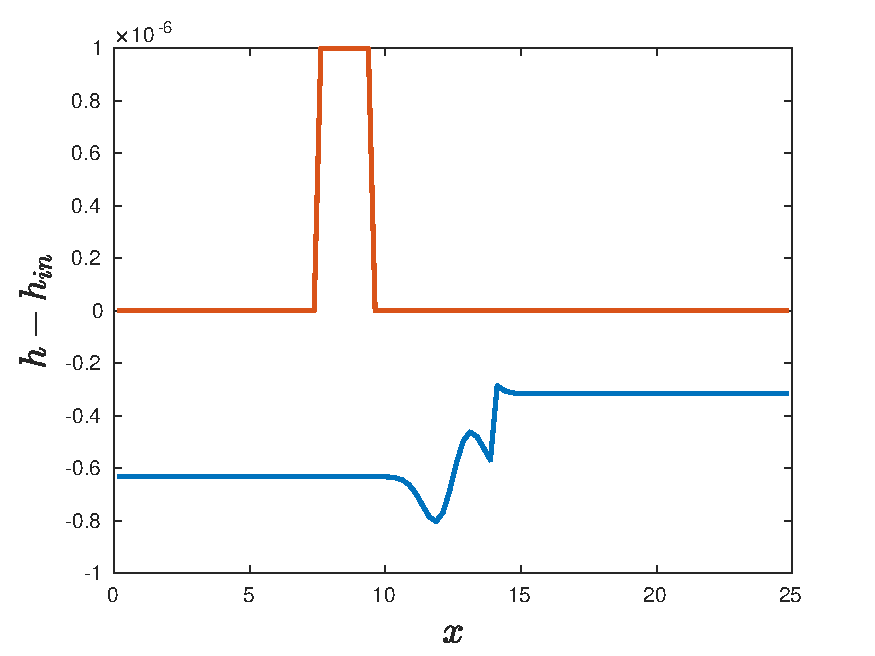
\includegraphics[width=0.9\textwidth]{figs/WENO-FD/figures/SW/Subcritical_discH/initial}
	\end{minipage}\hfill
	\begin{minipage}{0.5\textwidth}
		\centering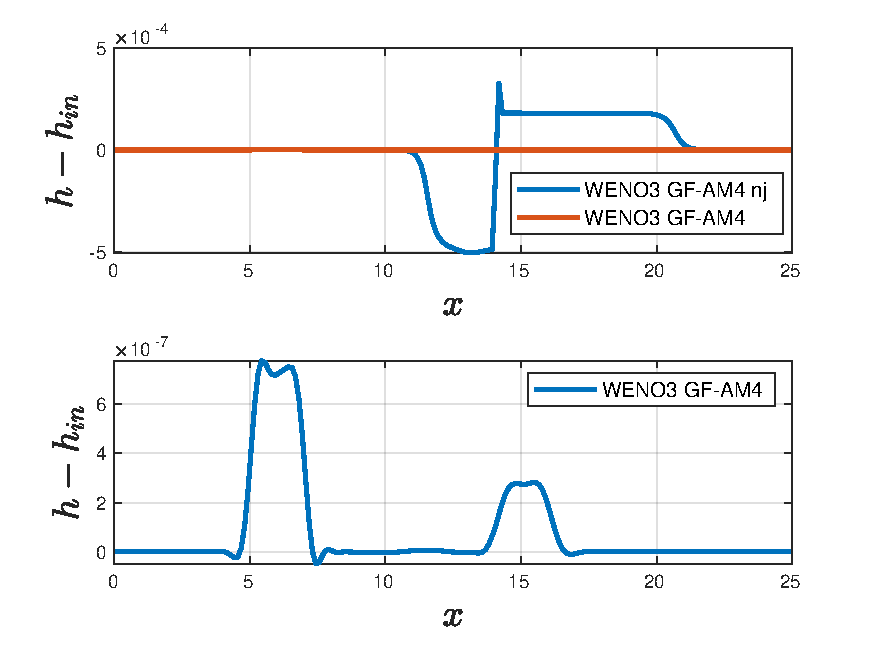
\includegraphics[width=0.9\textwidth]{figs/WENO-FD/figures/SW/Subcritical_discH/weno3_am4_n200} 
	\end{minipage}
}

\only<30>{
	\textbf{Subcritical flow with perturbation and Discontinuous H}\\
	\begin{minipage}{0.5\textwidth}
		\centering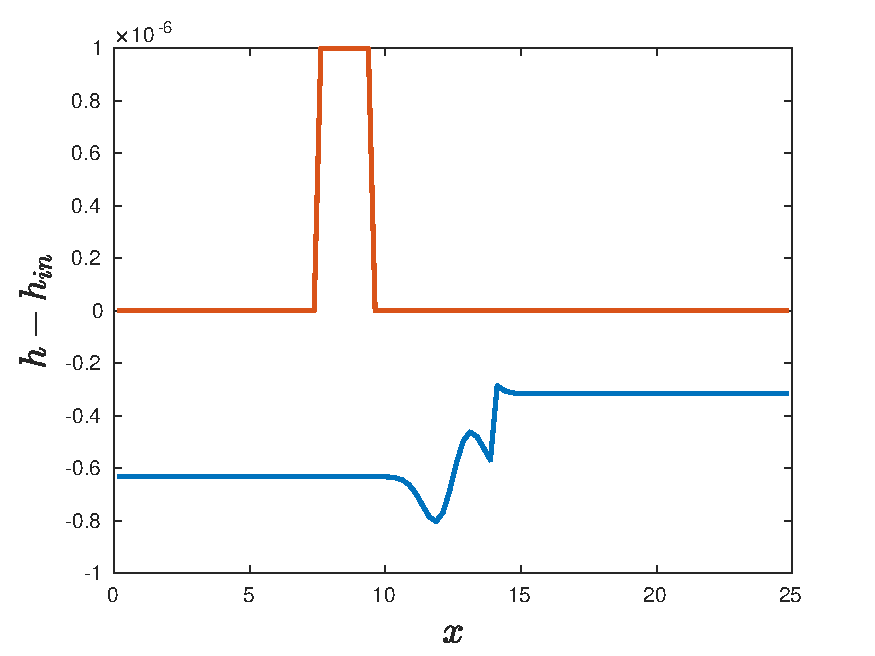
\includegraphics[width=0.9\textwidth]{figs/WENO-FD/figures/SW/Subcritical_discH/initial}
	\end{minipage}\hfill
	\begin{minipage}{0.5\textwidth}
		\centering\includegraphics[width=0.9\textwidth]{figs/WENO-FD/figures/SW/Subcritical_discH/weno3_am6_n200} 
	\end{minipage}
}
\end{frame}


\begin{frame}[t]{Global Flux Quadrature  with WENO approximation} 

\vspace{0.5cm}

\begin{enumerate}
\item[\textcolor{mblue1}{\Large\checkmark}] \textcolor{black}{No a-priori knowledge of equilibrium, all steady states!}    

\vspace{0.2cm}

\item[\textcolor{mblue1}{\Large\checkmark}] \textcolor{black}{No need of compute the solution of the Cauchy problem .. (maybe for initialization)}  

\vspace{0.2cm}

\item[\textcolor{mblue1}{\Large\checkmark}]  \textcolor{black}{Convergence at steady state arbitrarily accurate by changing ODE weights} 

\vspace{0.2cm}

\item[\textcolor{mblue1}{\Large\checkmark}]   \textcolor{black}{Discrete initial state can be generated}

\vspace{0.2cm}

\item[\textcolor{red}{\Large$\times$}]   \textcolor{black}{Non-compact quadrature }
\end{enumerate}


%\only<24>{
%	\centering\includegraphics[width=0.8\textwidth]{figs/GB.png} 
%}

\end{frame}
% 